\chapter{Neuronové sítě}
\label{sec:NN}

Umělá neuronová síť (ang. artificial neural network - ANN) nebo jen neuronová
síť (ang. neural network - NN) je výpočetní model inspirovaný biologickými
nervovými systémy v lidském mozku. Na rozdíl od konvenčních výpočetních modelů,
které zpracovávají informace algoritmicky, a tedy postupují dle předem určeného
postupu, se informace v tomto modelu šíří paralelně v síti vah mezi
jednotlivými neurony. Jelikož je výstup ze sítě dané architektury závislý
hlavně na numerických parametrech, zejména váhách jednotlivých spojů mezi
neurony, lze funkčnost sítě měnit bez změny programu pouhou změnou těchto
parametrů, a to i automaticky v procesu trénování modelu.

Nyní krátce projdeme historií vývoje neuronových sítí.

\section{Historie}
\label{sec:NN_History}

\subsection{Prvopočátky}
První matematický model neuronové sítě byl popsán v roce 1943 dvěma
neurofyziology - Warrenem McCullochem a Walterem Pittsem. \cite{McCulloch1943}
Model byl založen na síti jednoduchých logických prvků, které provedou vážený
součet svých vstupů a na výstup odešle signál založený na prahové funkcí.

V roce 1958 pak Frank Rosenblatt představil elektronický model neuronové sítě.
Základní jednotku, postavenou na McCulloch-Pittsově modelu, nazval perceptron.
\cite{Rosenblatt1958} Jeho architektura byla podobná modelu znázorněnému na
obrázku \ref{fig:neuron}, kde aktivační funkce je prahová funkce. Rosenblattův
stroj - Mark I Perceptron - byl postavený pro rozpoznávání jednoduchých vzorů v
obrazech. Hlavním omezením tohoto modelu bylo, že byl schopen rozlišovat pouze
lineárně separovatelné třídy. Samotný model perceptronu je dodnes používán jako
základ pro mnoho neuronových sítí.

Další systém - ADALINE (Adaptive Linear Neuron) - byl představen Bernardem
Widrowem a Tedym Hoffem v roce 1960. Tento model umělého neuronu byl velmi
podobný perceptronu, na rozdíl od něj ale neobsahoval prahovou ale lineární
funkci, výstup tedy nebyl binární ale spojitý. Pro učení pak byla využita
metoda nejmenších čtverců, která minimalizovala chybu mezi skutečným a
očekávaným výstupem. \cite{nn_history}

I když ve svých počátcích přitahoval koncept umělé inteligence mnoho vědců jako
i sponzorů, v následujících létech zájem ochabl, jelikož nebylo dosaženo
předpokládaných výsledků, hlavně s ohledem na tehdejší stav vývoje hardwaru a
obecně výpočetní techniky. Proto se tomuto období někdy říká Ai Winter.
Neznamená to ale, že ti, kteří se oboru nadále věnovali, nedosáhli významných
výsledků. \cite{nn_history}

\subsection{Backpropagation}
Významným milníkem v historii neuronových sítí byl objev algoritmu
backpropagation, zvaného taky algoritmus zpětného šíření chyby. Tento
algoritmus byl vyvinut v roce 1974 Paulem Werbosem, popularitu ale dosáhl až po
nezávislém objevení v roce 1986 Davidem Rumelhartem et al.
\cite{backpropagation}

Tento algoritmus umožnil trénovat sítě s více vrstvami, což položilo základ
hlubokému učení. Algoritmus využívá metodu gradientního sestupu v kombinaci s
řetězovým pravidlem derivací k nalezení optimálních vah sítě vedoucích k
minimalizaci chyby.

Vynález backpropagation byl jedním z hlavních důvodů, proč se v 80. letech
obnovil zájem o neuronové sítě a umělou inteligenci obecně. V 1989 roce taky
umožnil Yann LeCunovi at al. zefektivnit použití konvolučních neuronových sítí
pro rozpoznávání rukou psaných číslic \cite{lecun1989} a položit tak základ
širokému využití konvolučních sítí v oblasti počítačového vidění.

\section{Struktura neuronové sítě}

Umělé neuronové sítě jsou silně inspirované biologickými neuronovými sítěmi. A
i když napodobení celé funkčnosti lidského nervového systému by bylo velmi
složité - ne-li nereálné, zejména s ohledem na počet neuronů a způsob jejich
propojení, je možné simulovat alespoň některé funkce lidské mysli.

Pro provádění výpočtů využívají neuronové sítě distribuovaný, paralelní
přístup. Informace jsou tedy zpracovány, předávány a ukládány celou sítí,
nikoliv pomocí určitých paměťových buněk. Většina znalostí je uložena v silách
vazeb mezi jednotlivými neurony. Vazby, které vedou k úspěšnému řešení
problému, jsou posilovány, naopak ty, které vedou k neúspěchu, jsou oslabovány.

Podstatnou vlastností neuronových sítí je jejich schopnost učení. Tato
vlastnost způsobuje, že již není nutná algoritmizace řešené úlohy, ale stačí
neuronové síti opakovaně předložit příklady popisující daný problém, podle
kterých jsou postupně upravovány síly vazeb v síti. Tato fáze učení pak určuje,
jakým způsobem bude síť transformovat vstupní data na
výstupní.\cite{Vondrak1994}

\subsection{Neuron}
Biologický neuron se skládá ze tří hlavních částí. Dendrity přijímají vstupní
signály. V těle jsou vstupní signály sečteny do jednoho potenciálu, který vede
k vybuzení neuronu - zaslání signálu na výstup, pokud potenciál překročí
určitou mez. Axanové vlákno pak vede k synapsím, tedy spojům s dalšími neurony.
Lidská mysl pak funguje na principu posilování nebo oslabování těchto spojů.

Umělý neuron se snaží tuto funkčnost napodobit, viz obrázek \ref{fig:neuron}.
Jeho vstupy $x_i$ jsou násobeny váhami $w_i$, které reprezentují sílu daného
spoje. Neuron pak tyto vážené vstupy sečte, a na tento součet aplikuje
aktivační funkci (AF), která definuje hodnotu výstupu $y$. V prvním a základním
modelu neuronu, perceptronu, je AF prahová funkce s binárním výstupem. Nicméně
v praxi se dnes využívají většinou reálné hodnoty a AF je obvykle spojitá.
\cite{Vondrak1994} Existuje mnoho různých AF, některé z nich budou popsány v
další části.

Kromě vah jednotlivých vstupů neuron obvykle obsahuje ještě tzv. bias (někdy
taky práh nebo posun), jehož funkci je posunout vážený součet vstupů tak, aby
bylo možné modelovat i funkce, které nejsou nulové v počátku souřadnic. Je buď
reprezentován jako samostatný parametr, nebo jako váha konstantního vstupu s
hodnotou 1, jako na obrázku \ref{fig:neuron}.

Funkci umělého neuronu lze tedy formálně vyjádřit takto:

\begin{equation*}
    y=f\left(\sum_{i=0}^{n}w_{i}x_{i}\right)
\end{equation*}

kde $w_0$ je bias a $x_0=1$, anebo s osamostatněným biasem takto:

\begin{equation*}
    y = f\left(\sum_{i=1}^{n} w_i x_i + b\right)
\end{equation*}

kde $b$ je bias.

Obecně tvoří všechny vstupní váhy a bias množinu parametrů, které ovlivňují
funkčnost celé neuronové sítě. Proces trénování sítě pak spočívá v nalezení
optimálních hodnot těchto parametrů, které vedou k co nejmenší chybě při řešení
úlohy.

\begin{figure}[]
    \centering
    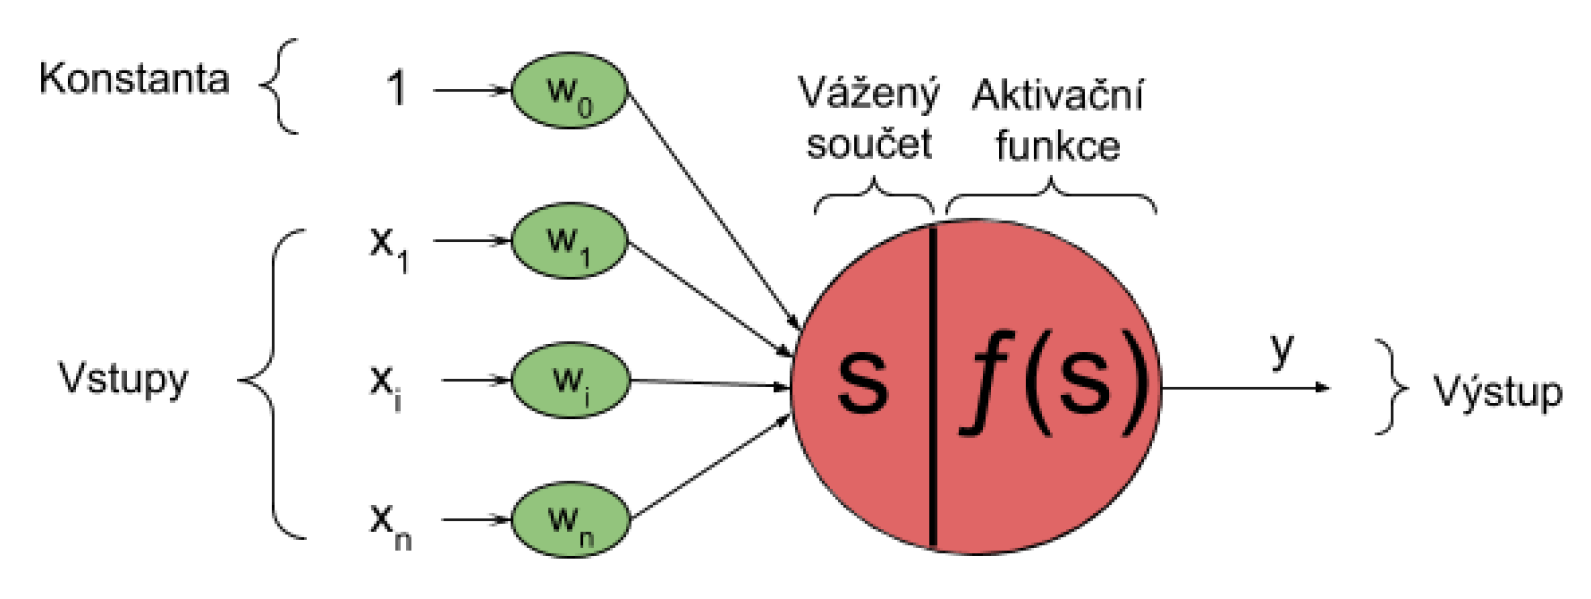
\includegraphics[width=0.5\textwidth]{Figures/neuron.png}
    \caption{Model umělého neuronu \cite{lagan}}
    \label{fig:neuron}
\end{figure}

\subsection{Základní aktivační funkce}

AF hraje stěžejní roli v umělých neuronových sítích zavedením nelinearity do
celého systému a umožňuje tak učení se složitějších vzorců.

V průběhu let bylo vyvinuto mnoho typů AF, a i když jejich úloha se zdá být
podobná, můžou se od sebe výrazně lišit. Jejich rozdíly spočívají zejména v
oboru hodnot, spojitosti, monotónnosti, a v tom, zda je závislá na přídavných
trénovaných parametrech. Ve výsledku se taky liší i jejich využití. Nyní
projdeme několik základních AF, od kterých se většina ostatních nějakým
způsobem odvíjí.

Sigmoida (lineární křivka) funkce transformuje vstup do rozmezí 0 ÷ 1, je tak
vhodná pro odhad pravděpodobnosti. Proto se taky někdy používá ve výstupních
vrstvách síti, zejména pro binární klasifikaci. Její funkčnost lze formálně
zapsat takto:

\begin{equation*}
    f(x)= \frac{1}{1+e^{-x}}
\end{equation*}

Její nevýhodou je hlavně problém mizejícího gradientu, kdy zejména ve
vícevrstvých sítích se velikost změn váh v počátečních a koncových vrstvách
významně liší. To pak způsobuje nestabilitu v procesu trénování a může jej
zpomalit nebo zcela zastavit. Navíc to, že není nulová v počátku souřadnic,
může způsobit špatnou konvergenci.

Hyperbolický tangens (tanh) je velmi podobný sigmoidě, ale transformuje vstup
do rozmezí -1 ÷ 1. Řeší tedy poslední zmíněný problém. Nicméně se pořád potýká
s problémem mizejícího gradientu. Taky, obě tyto funkce představují větší
výpočetní nároky. Formálně lze tuto AF popsat takto:

\begin{equation*}
    f(x)= \frac{e^x-e^{-x}}{e^x+e^{-x}}
\end{equation*}

ReLU (Rectified Linear Unit, taky někdy rampa) je jednoduchá a efektivní AF.
Pro kladné hodnoty se chová jako identita, pro záporné je nulová.

\begin{equation*}
    f(x)=\max(0,x)=\begin{cases}x&x>0,\\0&x\leq0,\end{cases}
\end{equation*}

Jelikož je výpočetně velmi nenáročná, je tato AF velmi oblíbená v hlubokých
sítích. Její nevýhodou ale je, že nezohledňuje záporné hodnoty, což v jejich
případě vede k problému mizejícího gradientu a může způsobit tzv. "mrtvé
neurony". Tento problém řeší různé varianty ReLU, jako například PReLU
(Parametric ReLU) nebo LReLU (Leaky ReLU). Tyto varianty přidávají parametr $p$
vynásobený $x$ pro záporné hodnoty:

\begin{equation*}
    f(x)=\max(0,x)=\begin{cases}x&x>0,\\p \cdot x&x\leq0\end{cases}
\end{equation*}

LReLU má tento parametr fixně nastavený na $p=0.01$, zatímco v případě PReLU je
tento parametr trénovaný spolu s jinými parametry sítě.

Další alternativou k ReLU je ELU (Exponential Linear Unit), která v záporné
části odpovídá exponenciální funkci:

\begin{equation*}
    f(x)=\begin{cases}x&x>0,\\a \left(e^{x}-1\right)&x\leq0\end{cases}
\end{equation*}

\begin{center}
    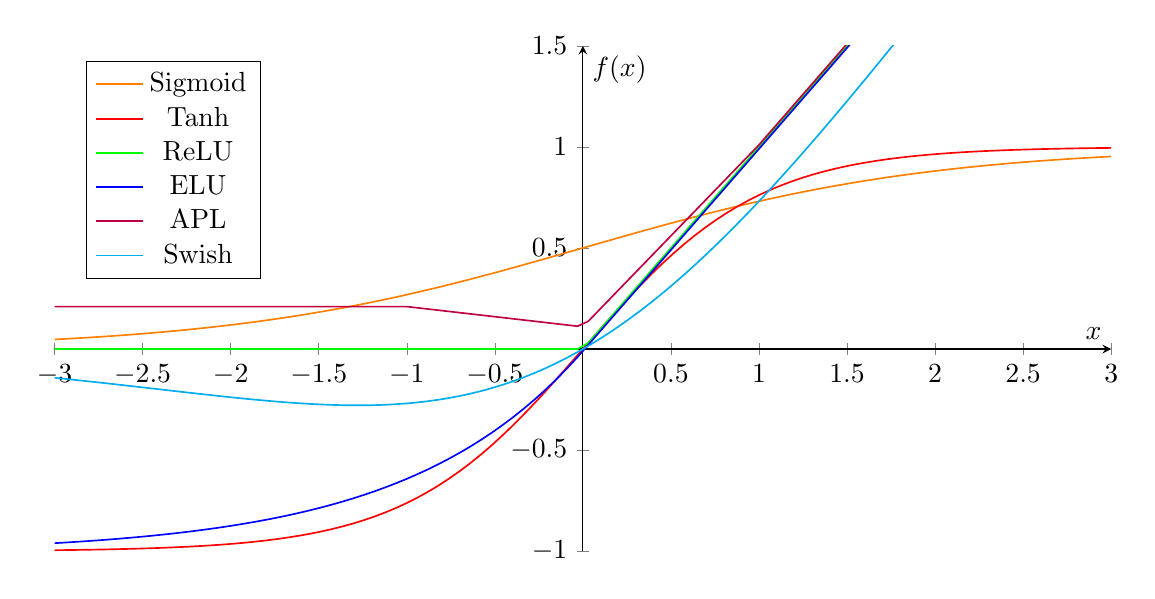
\begin{tikzpicture}
        \begin{axis}[
                axis lines=middle,
                xlabel={$x$},
                ylabel={$f(x)$},
                samples=100,
                domain=-3:3,
                legend pos=north west,
                ymin=-1, ymax=1.5,
                width=15cm, height=8cm
            ]
            % Sigmoid
            \addplot[orange, semithick] {1/(1+exp(-x))};
            \addlegendentry{Sigmoid}

            % Tanh
            \addplot[red, semithick] {tanh(x)};
            \addlegendentry{Tanh}

            % ReLU
            \addplot[green, semithick] {x*(x>0)};
            \addlegendentry{ReLU}

            % ELU (alpha = 1)
            \addplot[blue, semithick] {(x>0) * x + (x<=0) * (exp(x)-1) - 0.01};
            \addlegendentry{ELU}

            % APL (Adaptive Piecewise Linear) - using a simple approximation
            \addplot[purple, semithick] {max(0,x) + 0.1*min(0,x+1) - 0.1*min(0,x-1) + 0.01};
            \addlegendentry{APL}

            % Swish (x * sigmoid(x))
            \addplot[cyan, semithick] {x/(1+exp(-x))};
            \addlegendentry{Swish}

        \end{axis}
    \end{tikzpicture}
\end{center}

\subsection{Dělení neuronových sítí}

Neuronové sítě jsou dnes využívány v mnoha oblastech a dokážou řešit mnoho
různých úloh, nicméně neexistuje jediný typ sítě, který by dokázal řešit
všechny. V průběhu let proto bylo vyvinuto mnoho různých architektur sítí,
každá pro jiné využití.

Jedním ze základních způsobů, jak můžeme neuronové sítě rozdělit, je podle typu
učení: učení s učitelem (supervised) a učení bez učitele (unsupervised). V
případě učení s učitelem, předkládáme síti dvojice vstupů a očekávaných
výstupů, na jejichž základě se síť snaží minimalizovat chybu úpravou svých
parametrů. Oproti tomu, u učení bez učitele nemá síť k dispozici očekávané
výstupy, ale snaží se najít nějaké struktury v datech, například shluky. V
další části se budeme věnovat hlavně neuronovým sítím pro učení s učitelem.

Dále můžeme neuronové sítě rozdělit na dopředné (feedforward NN - FFNN) a
rekurentní (recurrent NN - RNN). U dopředných sítí se informace šíří pouze ze
vstupu k výstupu a nevyskytují se žádné smyčky. Naopak rekurentní sítě obsahují
zpětnou vazbu z výstupu přivedenou na vstup. To umožňuje reagovat na změny v
čase.

Další možnosti jejich rozdělení je dle topologie, která zahrnuje jejich
hloubku, tzn. počet vrstev, velikost těchto vrstev a jejich vzájemné propojení.
V další sekci se budeme věnovat právě uspořádání vrstev v neuronových sítích.

\section{Topologie neuronových sítí}
Nejčastější uspořádání neuronů v neuronových sítích je do vrstev. Neurony dané
vrstvy jsou spojeny pouze s neurony z předchozí a následující vrstvy. Vrstvy
pak dělíme na tři typy: vstupní, výstupní a skryté. Vstupní vrstva neobsahuje
neurony a neprovádí žádné operace, pouze přijímá vnější signály a distribuuje
je do další vrstvy. Výstup z neuronů ve výstupní vrstvě pak reprezentuje výstup
celé sítě.

Pokud síť obsahuje pouze vstupní a výstupní vrstvu, mluvíme o jednovrstvé
neuronové síti. Takové sítě mají velmi omezené možnosti, proto se v praxi
nepoužívají. Většina neuronových sítí má mezi vstupní a výstupní vrstvou
alespoň jednu skrytou vrstvu, viz obrázek \ref{fig:layers}.

U většiny klasických dopředných neuronových sítí jsou jednotlivé vrstvy mezi
sebou plně propojeny, tzn. každý prvek jedné vrstvy je propojený se všemi prvky
následující vrstvy.

\begin{figure}[]
    \centering
    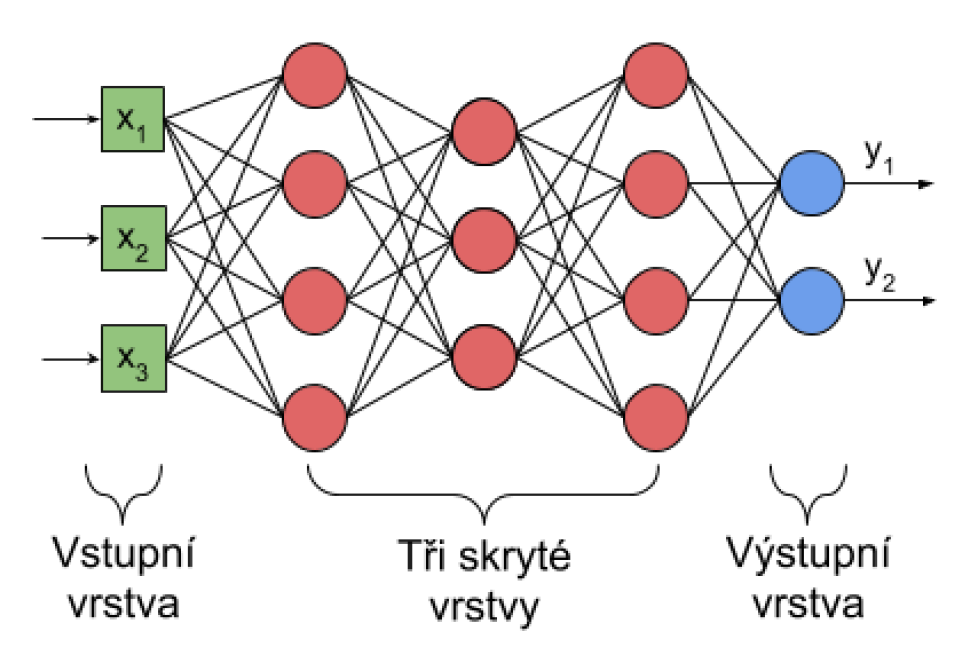
\includegraphics[width=0.5\textwidth]{Figures/layers.png}
    \caption{Vícevrstvá, plně propojená síť \cite{lagan}}
    \label{fig:layers}
\end{figure}

\section{Proces trénování s využitím backpropagation}

Jak již bylo řečeno, proces trénování NN spočívá v nalezení optimálních hodnot
parametrů jednotlivých neuronů. Optimální parametry pak vedou k minimální
chybě. Chybou rozumíme rozdíl mezi skutečným výstupem sítě a očekávaným
výstupem. K tomu se nejčastěji používá algoritmus backpropagation (taky
Algoritmus zpětného šíření chyby). Nyní si popíšeme, jak trénování sítě pomocí
tohoto algoritmu funguje.

Nejprve se ze vstupních dat vypočítají pomocí aktuálních parametrů sítě reálně
výstupy sítě. Tento proces se nazývá dopředný průchod (ang. forward pass).
Následně se pomocí chybové funkce (ang. loss function, taky nákladová funkce -
ang. loss function) spočítá chyba sítě. Ta vyjadřuje, v jaké míře se skutečné
výstupy liší od očekávaných. Můžou být použity různé chybové funkce, v
závislosti na typu úlohy, kterou síť řeší.

V klasifikačních úlohách je nejčastěji používaná chybová funkce křížové
entropie, která porovnává rozdělení pravděpodobnosti skutečného výstupu sítě s
očekávaným rozdělením pravděpodobnosti. Pro regresní úlohy se používá například
střední kvadratická chyba (ang. mean squared error - MSE) vyjadřující střední
hodnotu druhých mocnin rozdílů mezi skutečnými a očekávanými hodnotami. Další
možností je absolutní chyba (ang. mean absolute error - MAE), která vyjadřuje
střední hodnotu absolutních hodnot rozdílů.

Dále je používaná metoda gradientního sestupu, k nalezení minima chybové
funkce. Za tímto účelem se vypočítají derivace chyby podle jednotlivých
parametrů sítě. Tyto derivace pak určují, jakým směrem a jak rychle se mají
dané parametry měnit, aby se chyba minimalizovala. Jelikož se derivace
parametrů v dané vrstvě vypočítávají pomocí řetězového pravidla derivací podle
derivací parametrů následující vrstvy, je tento proces nazýván zpětný průchod
(ang. backward pass).

Jednotlivé parametry se pak podle vypočítaných derivací upraví. Velikost změny
je určená hyperparametrem rychlostí učení (ang. learning rate, taky krok),
který určuje, jak rychle se mají parametry měnit. Vypočítaná derivace se
vynásobí rychlostí učení a přičte k původní hodnotě parametru. Tento proces se
opakuje pro všechny parametry sítě. Metoda gradientního sestupu umožňuje větší
změny parametrů, když jsou daleko od minima - absolutní hodnoty derivací jsou
větší, a naopak menší změny, když se k němu blíží - derivace se blíží nule.

Proces trénování sítě se skládá z opakování dopředného a zpětného průchodu pro
všechna trénovací data (někdy postupně pro jejich podmnožiny - dávky, ang.
batches). Po každém průchodu se upraví parametry sítě podle vypočítaných
derivací. Tento proces se opakuje, dokud chyba nedosáhne požadované úrovně,
nenastane její konvergence nebo není překročen maximální počet iterací.

\section{Optimalizace procesu trénování}

V základní verzi algoritmu backpropagation se využívá výše popsaný gradientní
sestup. Ten ale může mít některé problémy, které mohou zpomalit proces
trénování nebo jej někdy zcela znemožnit. Nyní si popíšeme některé z těchto
problémů a jejich možná řešení.

Jedním z podstatných problémů gradientního sestupu je, že se může lehce
zaseknout v lokálním minimu, kde je derivace nulová. To může způsobit, že se
síť zastaví v nějakém suboptimálním bodě a nepokračuje do globálního minima,
které by odpovídalo optimálnímu řešení. Tento problém se často řeší přidáním
tzv. momentu do úpravy parametrů. Tento proces bere v úvahu i předchozí změny
parametrů. V případě, že se derivace parametru v průběhu trénování změní,
moment umožňuje parametrům ještě nějakou dobu pokračovat v pohybu ve stejném
směru. To většinou pomůže překonat lokální minima a dosáhnout tak globálního
minima.

Dalším řešením tohoto problému je využití stochastické aproximace gradientního
sestupu (ang. stochastic gradient descent - SGD), kde se gradient počítá pro
náhodně vybrané podmnožiny trénovacích dat. Tento postup umožňuje rychlejší
konvergenci, počítáme totiž gradient jen pro část dat, a zároveň zabraňuje
zaseknutí v lokálním minimu zavedením šumu do procesu trénování. Tato metoda se
využívá nejčastěji pro velké datasety.

Dalším problémem může být nastavení optimálního kroku učení. Pokud je krok
příliš velký, může dojít k příliš velké změně, která opomine minimum, můžeme
tak nikdy nedosáhnout konvergence. Naopak, pokud je krok příliš malý, může
trénování trvat příliš dlouho. Řešením může být například adaptivní nastavení
kroku. Nejznámější taková metoda je RMSProp (ang. root mean square
propagation), která upravuje krok učení pro každý parametr podle průměrného
druhého momentu gradientu. Další možností je v průběhu trénování postupně
snižovat krok (ang. learning rate decay).

Populárním řešením těchto problémů je také Adam (ang. adaptive moment
estimation, v překladu adaptivní odhad momentu), který kombinuje zavedení
momentu a adaptivního nastavení kroku pomocí RMSProp.

Další metodou, jak optimalizovat nastavení kroku, je normalizace dat mezi
vrstvami sítě (ang. batch normalization). Tím se zamezí příliš velkým změnám v
jednotlivých vrstvách, které někdy destabilizují proces trénování.

U trénování hlubokých sítí se často naráží také na problém přetrénování (taky
nadměrné přizpůsobení, ang. overfitting). Přetrénování nastává, když se síť
dobře naučí trénovací data, zároveň ale postrádá schopnost generalizace, a když
pak dostane nová data, nedosahuje dobrých výsledků. K základním řešením tohoto
problému patří použití většího množství trénovacích dat - pokud jsou dostupná,
jinak se někdy zavádí umělé variace dat jako rotace či převrácení, jinak je
třeba někdy zvážit zjednodušení architektury modelu. Dále pak jsou využívány
techniky regularizace, které upravují samotný proces trénování.

Nejjednodušší regularizační technikou je tzv. předčasné zastavení, tedy
zastavení trénování v případě, že se chyba na validačních datech začne
zvyšovat. Další možností je dropout (taky výpadek), kdy se u určitého počtu
náhodně zvolených neuronů v průběhu trénování nastaví na výstupu nula. Tím se
snižuje závislost sítě na konkrétních neuronech a zvyšuje se tak její schopnost
generalizace.

Další dvě metody, nazývané L1 a L2 regularizace, přičítají k chybové funkci
člen, který penalizuje velikost parametrů sítě. L1 regularizace (taky metoda
Lasso, z ang. least absolute shrinkage and selection operator) přičítá k
chybové funkci součet absolutních hodnot všech parametrů sítě vynásobený
hyperparametrem, který určuje míru této penalizace. Tato metoda vede k řídké
síti, ve které je mnoho parametrů nulových. L2 regularizace (taky hřebenová
regrese, ang. ridge regression) přičítá k chybové funkci součet druhých mocnin
všech parametrů sítě vynásobený hyperparametrem $\lambda$. Tato metoda vede
jednak k menší variabilitě parametrů, jednak k pomalejším změnám parametrů v
průběhů trénování, v důsledku pak k menší citlivosti na šum v datech. Využívá
se zejména v hlubokých sítích.

\endinput